%%%%%%%%%%%%%%%%%%%%%%%%%%%%%%%%%%%
%This is the LaTeX ARTICLE template for RSC journals
%Copyright The Royal Society of Chemistry 2016
%%%%%%%%%%%%%%%%%%%%%%%%%%%%%%%%%%%

\documentclass[twoside,twocolumn,9pt]{article}
\usepackage{extsizes}
\usepackage[super,sort&compress,comma]{natbib} 
\usepackage[version=3]{mhchem}
\usepackage[left=1.5cm, right=1.5cm, top=1.785cm, bottom=2.0cm]{geometry}
\usepackage{balance}
\usepackage{mathptmx}
\usepackage{sectsty}
\usepackage{graphicx} 
\usepackage{lastpage}
\usepackage[format=plain,justification=justified,singlelinecheck=false,font={stretch=1.125,small,sf},labelfont=bf,labelsep=space]{caption}
\usepackage{float}
\usepackage{fancyhdr}
\usepackage{fnpos}
\usepackage[english]{babel}
\addto{\captionsenglish}{%
  \renewcommand{\refname}{Notes and references}
}
\usepackage{array}
\usepackage{droidsans}
\usepackage{charter}
\usepackage[T1]{fontenc}
\usepackage[usenames,dvipsnames]{xcolor}
\usepackage{setspace}
\usepackage[compact]{titlesec}
\usepackage{hyperref}
%%%Please don't disable any packages in the preamble, as this may cause the template to display incorrectly.%%%


\usepackage{epstopdf}%This line makes .eps figures into .pdf - please comment out if not required.

\definecolor{cream}{RGB}{222,217,201}

\usepackage{layout}

\begin{document}

\pagestyle{fancy}
\thispagestyle{plain}
\fancypagestyle{plain}{
%%%HEADER%%%
\renewcommand{\headrulewidth}{0pt}
}
%%%END OF HEADER


%%%PAGE SETUP - Please do not change any commands within this section%%%
\makeFNbottom
\makeatletter
\renewcommand\LARGE{\@setfontsize\LARGE{15pt}{17}}
\renewcommand\Large{\@setfontsize\Large{12pt}{14}}
\renewcommand\large{\@setfontsize\large{10pt}{12}}
\renewcommand\footnotesize{\@setfontsize\footnotesize{7pt}{10}}
\makeatother

\renewcommand{\thefootnote}{\fnsymbol{footnote}}
\renewcommand\footnoterule{\vspace*{1pt}% 
\color{cream}\hrule width 3.5in height 0.4pt \color{black}\vspace*{5pt}} 
\setcounter{secnumdepth}{5}

\makeatletter 
\renewcommand\@biblabel[1]{#1}            
\renewcommand\@makefntext[1]% 
{\noindent\makebox[0pt][r]{\@thefnmark\,}#1}
\makeatother 
\renewcommand{\figurename}{\small{Fig.}~}
\sectionfont{\sffamily\Large}
\subsectionfont{\normalsize}
\subsubsectionfont{\bf}
\setstretch{1.125} %In particular, please do not alter this line.
\setlength{\skip\footins}{0.8cm}
\setlength{\footnotesep}{0.25cm}
\setlength{\jot}{10pt}
\titlespacing*{\section}{0pt}{4pt}{4pt}
\titlespacing*{\subsection}{0pt}{15pt}{1pt}
%%%END OF PAGE SETUP%%%

%%%FOOTER%%%
\fancyfoot{}
\fancyfoot[LO,RE]{\vspace{-7.1pt}
\includegraphics[height=9pt]{auxiliary/rsc_template_head_foot/LF}}
\fancyfoot[CO]{\vspace{-7.1pt}\hspace{13.2cm}
\includegraphics{auxiliary/rsc_template_head_foot/RF}}
\fancyfoot[CE]{\vspace{-7.2pt}\hspace{-14.2cm}
\includegraphics{auxiliary/rsc_template_head_foot/RF}}
\fancyfoot[RO]{\footnotesize{\sffamily{1--\pageref{LastPage} ~\textbar  \hspace{2pt}\thepage}}}
\fancyfoot[LE]{\footnotesize{\sffamily{\thepage~\textbar\hspace{3.45cm} 1--\pageref{LastPage}}}}
\fancyhead{}
\renewcommand{\headrulewidth}{0pt} 
\renewcommand{\footrulewidth}{0pt}
\setlength{\arrayrulewidth}{1pt}
\setlength{\columnsep}{6.5mm}
\setlength\bibsep{1pt}
%%%END OF FOOTER%%%

%%%FIGURE SETUP - please do not change any commands within this section%%%
\makeatletter 
\newlength{\figrulesep} 
\setlength{\figrulesep}{0.5\textfloatsep} 

\newcommand{\topfigrule}{\vspace*{-1pt}% 
\noindent{\color{cream}\rule[-\figrulesep]{\columnwidth}{1.5pt}} }

\newcommand{\botfigrule}{\vspace*{-2pt}% 
\noindent{\color{cream}\rule[\figrulesep]{\columnwidth}{1.5pt}} }

\newcommand{\dblfigrule}{\vspace*{-1pt}% 
\noindent{\color{cream}\rule[-\figrulesep]{\textwidth}{1.5pt}} }

\makeatother
%%%END OF FIGURE SETUP%%%

%%%TITLE, AUTHORS AND ABSTRACT%%%
\twocolumn[
  \begin{@twocolumnfalse}
{
\includegraphics[height=30pt]{auxiliary/rsc_template_head_foot/journal_name}\hfill\raisebox{0pt}[0pt][0pt]{
\includegraphics[height=55pt]{auxiliary/rsc_template_head_foot/RSC_LOGO_CMYK}}\\[1ex]

\includegraphics[width=18.5cm]{auxiliary/rsc_template_head_foot/header_bar}}\par
\vspace{1em}
\sffamily
\begin{tabular}{m{4.5cm} p{13.5cm} }


\includegraphics{auxiliary/rsc_template_head_foot/DOI} & \noindent\LARGE{\textbf{Rapid technological progress in white light-emitting diodes and its sources in innovation and technology spillovers}} \\
\vspace{0.3cm} & \vspace{0.3cm} \\

 & \noindent\large{Michael Weinold \textit{$^{a b \ddag}$}, Sergey Kolesnikov,\textit{$^b$} and Laura Diaz Anadon\textit{$^{b}$}} \\

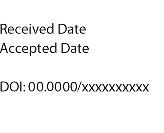
\includegraphics{auxiliary/rsc_template_head_foot/dates} & \noindent\normalsize{First commercial white light-emitting diodes (LEDs) were introduced to the market in 1996. Since then, white LEDs have experienced major improvements in performance and decreases in cost, resulting in rapid market expansion of LED-based solid-state lighting (SSL), one of the key current solutions in global climate change mitigation efforts. Despite the significance of the technology, the extent and sources of these improvements have not been systematically investigated. Understanding what has driven rapid progress in LEDs can provide lessons for accelerating innovation in a broad range of other demand-side clean energy technologies for climate change mitigation. With this aim, we gather systematic evidence on cost and performance improvements in white LEDs from a literature review, interviews with experts in industry and academia, and cost and performance modelling. We find that the overall efficiency of the highest performing warm white LED packages has improved from $\eta_L=5.8\%$ in 2003 to $\eta_L=38.7\%$ in 2020. During the same period, we estimate that the cost of manufacturing low-power and mid-power LED packages at a U.S. location using state-of-the-art equipment has dropped from 1.1\$ to 0.05\$ (in 2020 USD) between 2003 and 2020, a 95.5\% decrease. We also show that technology spillovers — i.e., knowledge originating in other technologies—affected all performance dimensions of LEDs, contributing no less than 8.5\% of the total efficiency improvements and $\sim$100\% of the improvements in consumer experience metrics. The increase in wafer size and manufacturing yield improvements were the primary causes of LED manufacturing cost reductions.}

\end{tabular}

 \end{@twocolumnfalse} \vspace{0.6cm}

  ]
%%%END OF TITLE, AUTHORS AND ABSTRACT%%%

%%%FONT SETUP - please do not change any commands within this section
\renewcommand*\rmdefault{bch}\normalfont\upshape
\rmfamily
\section*{}
\vspace{-1cm}


%%%FOOTNOTES%%%

\footnotetext{\textit{$^{a}$~ETH Zurich, Zurich, Switzerland. E-mail: michael.weinold@alumni.ethz.ch}}
\footnotetext{\textit{$^{b}$~Cambridge Centre for Environment, Energy and Natural Resource Governance, Department of Land Economy, University of Cambridge, Cambridge, United Kingdom. }}

%Please use \dag to cite the ESI in the main text of the article.
%If you article does not have ESI please remove the the \dag symbol from the title and the footnotetext below.
\footnotetext{\dag~Electronic Supplementary Information (ESI) available: [details of any supplementary information available should be included here]. See DOI: 00.0000/00000000.}
%additional addresses can be cited as above using the lower-case letters, c, d, e... If all authors are from the same address, no letter is required

\footnotetext{\ddag~Present address: Paul Scherrer Institut, Laboratory for Energy Analysis, Group for Technology Assessment, Switzerland.}


%%%END OF FOOTNOTES%%%

%%%MAIN TEXT%%%%

\section{Introduction}

A rapid reduction of global carbon dioxide emissions is urgently required in order to mitigate the effects of climate change \cite{Forster2019}. According to the United Nations, by the end of 2021, more than 130 countries have set or are considering setting a net zero emissions target by or around 2050 \cite{un2021climate}. The European Union, for example, has set a goal of net zero emissions by 2050—a goal it aims to meet with the help of the European Green Deal, alongside other EU and national policies \cite{eu2020green}. The United Kingdom similarly has adopted a similar strategy to achieve net-zero by 2050 \cite{noauthor_ieairena_2023}.

Achieving these ambitious and critically important targets will require both the deployment of new clean energy technologies, and the acceleration of innovation in existing supply-side \cite{sinn2012green} and demand-side energy technologies \cite{rgeVorsatz2009}. To ensure rapid adoption of these technologies, significant reductions in their costs and improvements in their performance and consumer experience are needed. This requires understanding how these cost reductions and performance improvements can be achieved \cite{Stephan2021} \cite{Ziegler2021}.

There are a range of mechanisms that contribute to improvements in a technology over time, including targeted research and development (R\&D) efforts, economies of scale, learning by doing \cite{Arrow1971}, and economies of scope \cite{johansson2012global}\cite{national2016power}\cite{iea2020perspectives}. The role of these factors at different stages of the innovation life cycle \cite{ grubler2012policies}, from research and technology development to demonstration, market formation and diffusion, is an area of active research \cite{Mowery1979} \cite{kavlak2018evaluating} \cite{Ziegler2021}. Innovation is also driven by forces of supply and demand. Various \textit{"technology-push"} drivers reduce the costs of innovating, while \textit{"market-pull"} drivers increase the pay-offs from investing in innovation \cite{anadon2009policy}.

\begin{figure*}[h]
 \centering
 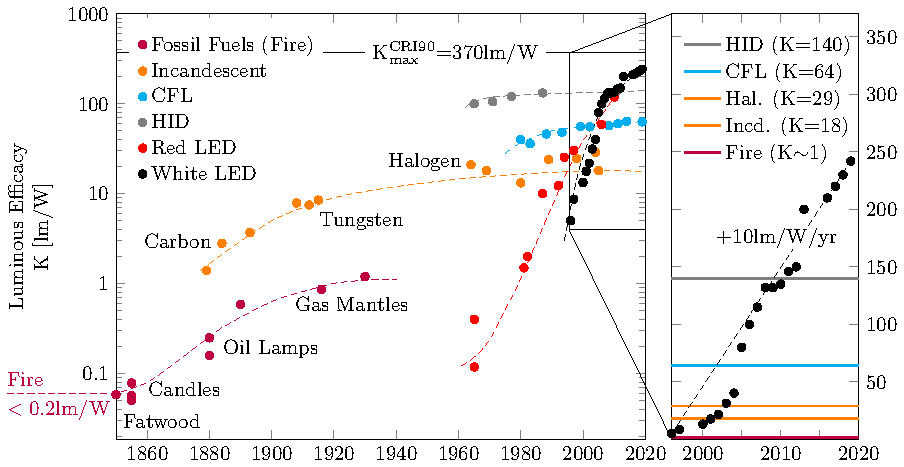
\includegraphics[height=7cm]{2_SSL_EES/article/figures/history_efficacy.pdf}
 \caption{Historical development of the luminous efficacy ($K$) of the most widely-used lighting technologies in human history from 1850 to 2020. Data shown for best performers by year of market introduction, with dashed lines. A multi-order polynomial fit was used to indicate the average rate of change as dashed lines. The physical limit for an ideal light source with a colour rendering index of CRI=90, denoted as $K_max^{CRI90}$, is shown as a black horizontal line, as per calculations by Murphy et al. \cite{Murphy2012}. The magnified plot shows the progress in cool white LEDs from 1996 to 2020, with the dashed line indicating a linear rate of efficacy improvement of 10lm/W per year. For comparison, efficacies of best performers in legacy lighting technologies for 2020 are shown as coloured horizontal lines. Note the logarithmic scale of the vertical axis on the main plot and the linear scale on the magnified plot. Abbreviations: HID – High-Intensity Discharge; CFL – Compact Fluorescent Lamp; Hal. – Halogen, Incd. – Incandescent. Source: own synthesis of published data based on a visual approach proposed by Azevedo et al. \cite{azevedo2009transition}. See Supplementary Information, section , for the full list of data sources. }
 \label{fgr:history_efficacy}
\end{figure*}
 
 
The stages and drivers of the innovation life-cycle for a particular technology play out within a broader innovation system \cite{grubler2012policies}\cite{Anadon2016}. Among these drivers, the role of external  knowledge transfer and technology spillovers in research and development of energy technologies is an understudied area  \cite{Stephan2021}. While the exact definition of spillovers in literature depends on the context and the research question \cite{Liu2003}\cite{Nemet2012}, we follow Stephan et al. \cite{Stephan2021} and consider knowledge to be external – thus a spillover –  if it has been developed for application in other technologies, sectors, or scientific disciplines. There is emerging evidence that understanding spillovers and the knowledge network outside a technology may be an important factor in understanding \cite{Pichler2020} and shaping \cite{Clark2016}\cite{Stephan2021}\cite{Sun2021}\cite{kolesnikov_framework_2022} the future evolution of technologies.  

Among demand-side technologies, the provision of lighting is a particularly important area for climate change mitigation efforts, as it currently   accounts for 15-19\% of global electricity consumption \cite{Zissis2016}\cite{doe_electricity}. It is also an area of rapid recent technological change: since the introduction of the first commercial white light-emitting diodes (LEDs) in 1996, lighting technology has experienced dramatic efficiency improvements.  As shown in Figure \ref{fgr:history_efficacy}, thanks to the introduction of LED-based solid-state lighting (SSL), the efficacy of lighting sources has increased by three orders of magnitude in just over 20 years , which is significantly faster than the historical progress observed in previous lighting technologies \cite{weinold2021quantifying}. For comparison, the highest performing light-emitting devices today reach efficacies of 220 lm/W \cite{lumistrips2021mid}, while an incandescent light bulb can only reach efficacies of up to 18 lm/W. Moreover, this rapid improvement in efficiency has been accompanied by a similarly impressive decrease in LED manufacturing costs and retail prices. Figure \ref{fgr:cost_lamp_small} shows how LED retail prices have fallen by two orders of magnitude, at an annual price per flux decline during the period of from 2008-2020 of 27.3\%, in line with previous estimates \cite{Gerke2020}.  


\begin{figure}
\centering
  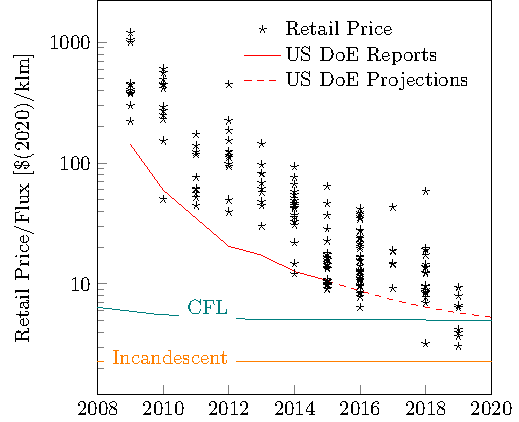
\includegraphics[height=5cm]{2_SSL_EES/article/figures/cost_lamp_small.pdf}
  \caption{Historical development of retail sales prices (in 2020 USD) per luminous flux of LED-based luminaires, including light bulbs, spotlights and recessed lights from 2008 to 2020. Red curved and dashed lines represent average retail sales prices and price projections for LED based luminaires published by the U.S. Department of Energy (DoE) \cite{council2013assessment}. Shown for reference are the average prices for compact fluorescent (CFL) and incandescent light bulbs. Source: own synthesis of data on LED sales prices collected from various consumer watchdog databases and publications. Data on CFL sales prices collected from \cite{eger2018origin} as well as various consumer watchdog databases and publications. Incandescent light bulb price is assumed constant based on the average in the covered time period. See Supplementary information, section …, for the full list of data sources.}
  \label{fgr:cost_lamp_small}
\end{figure}

These  dramatic improvements in lighting technology, supported by the introduction of lighting efficiency regulations phasing out incandescent lightbulbs and targeted policies stimulating LED adoption in many countries, led to the rapid expansion and diffusion of SSL technologies  \cite{weinold2020long}\cite{Mills2014}\cite{Stegmaier2021}\cite{grubb2021new}. As a result, by 2020, highly efficient LED luminaires were saving an estimated 131 TWh/year for the EU \cite{eu2019impactass} and 442 TWh/year for the US \cite{guidehouse2020adoption}, which is on par with the amount of energy produced annually by all solar photovoltaic installations in these regions. Notably, market adoption of LED lighting is not limited to developed economies \cite{Kamat2020}. For example, durability, low up-front cost and high efficiency of LED light sources have led to their wide-spread adoption in rural West African communities without access to grid electricity \cite{Bensch2017}. LEDs have also been used in a wide range of applications beyond lighting, such as personal health monitors \cite{o2019optical}, \cite{Wyatt2020}, watches and smartphones \cite{Bai2017}, potable water treatment \cite{Lui2014}, high-bandwidth wireless data transmission \cite{Haas2016}, and augmented reality eye wear \cite{Lee2016}. 

Despite this impressive history, the sources of LED innovation have not received as much attention from researchers as innovation in supply-side  energy technologies, such as solar photovoltaics  \cite{kavlak2018evaluating} or wind energy \cite{qiu2012price}\cite{jennings2020policy}, or in lithium-ion batteries for transportation \cite{Ziegler2021}\cite{Stephan2021}. To the best of our knowledge, no study has comprehensively discussed the sources or extent of progress across various metrics of LED cost or performance since the introduction of first commercial white LED products.  Understanding the extent to which individual innovations and knowledge spillovers  contributed to improvements in LED technology, how this effect compares to other sources of improvements such as economies of scale, and how these innovations occurred (i.e., by what mechanisms and actors) will provide valuable lessons both for other demand-side technologies and overall for accelerating clean energy innovation.

To address these questions, in this paper we identify a set of metrics suitable for tracking the historical progress of LED lighting technology. We then trace device efficiency and cost improvements, as well as changes in relevant consumer experience metrics from the time of introduction of the first commercial warm white LEDs in 2003 to 2020, the year with the most recent data available at the time of writing  . Given the proprietary nature of knowledge in the SSL industry , we collect corresponding information using a multi-method approach combining a systematic literature review of scientific literature and industry reports with patent analysis and a series of elite interviews \cite{Tansey} with eminent experts from academia, public research institutions and industry. This approach allows us to identify innovations in white LED technology and examine their origins to discern technology spillovers among them. Data on performance improvements associated with individual innovations identified in patents, scientific publications, industry reports, and interviews is then augmented  by our calculations of device efficiency, including contributions of specific spillovers to the overall LED efficiency (see Supplementary Information for more detail). We further calculate LED manufacturing costs using own bottom-up cost model with a process-step resolution. Finally, we discuss what our observations and conclusions mean for the understanding of the innovation process in LED technology and for broader policy and industry efforts to accelerate clean energy innovation.

\section{Previous literature}

The historical development of light-emitting diodes has received a considerable amount of attention following the recognition of pioneering work on blue LED by Japanese researchers Shuji Nakamura, Isamu Akasaki and Hiroshi Amano with the 2014 Nobel Prize in Physics \cite{Akasaki2015} \cite{Nakamura2015}. The sources and disaggregated contributions of subsequent improvements in LED technology, however, have not been documented in the literature in a systematic fashion, though there were notable publications reporting on the progress in the design of devices \cite{Shchekin2006} \cite{krames2007led} \cite{laubsch2009high} \cite{hahn2014development}, or contributions of different sub-efficiencies to overall device efficiency for 2009 \cite{tsao2010solid} and 2016 \cite{pattison2017solid}. 

Several descriptive papers include very useful information on some of the scientific breakthroughs that have contributed to LED progress \cite{krames2007status}, \cite{Phillips2007}, \cite{Bierhuizen2007}, \cite{Nakamura2013}, \cite{feezell2018invention} and \cite{Taki2019}. Additional  studies providing more detail on specific advances in LED technology were also published by authors working for key industry actors Lumileds\cite{MuellerMach2005}, \cite{Shchekin2006}, \cite{lumi2015lumi}, \cite{Bhardwaj2017} and Osram (now amsOsram) \cite{Haerle2004}, \cite{Baur2009}, \cite{laubsch2009high}, \cite{hahn2014development}. However, these studies typically include limited information on the macro chip-design and cover disparate aspects of the technology over different time periods. Another important source of historical information comes from patents, which cover the entirety of the device architecture or manufacturing process, including those by Lumileds \cite{margalith2011thin}, Samsung \cite{jung2014phos} \cite{cha2019semiconductor} and Soraa \cite{cich2017high}.

We summarize the information collected, analysed and classified on the progress in LED chip architectures and manufacturing processes from these and other disparate sources in Figure 3, where we show the evolution of LEDs from classical chips with lateral current spreading to chip-scale package flip-chip architectures. Despite the amount of literature published on the topic of LED history, to the best of our knowledge, no publication comprehensively aggregates known chip design, manufacturing, and material improvements to show the overall effect of these improvements on device efficiency or manufacturing cost over time. In addition, the effect of individual innovations and technology spillovers, which has been investigated in solar PV \cite{kavlak2018evaluating} \cite{kolesnikov2020novel} \cite{nemet2019solar}, and to some extent in lithium-ion batteries \cite{Stephan2021}, has not been studied in the context of lighting yet. This is consistent with previous observations regarding the marginalization of end-use technologies in the analysis of energy innovation for climate change impact mitigation \cite{Wilson2012}, \cite{Creutzig2018}.


\begin{figure*}
 \centering
 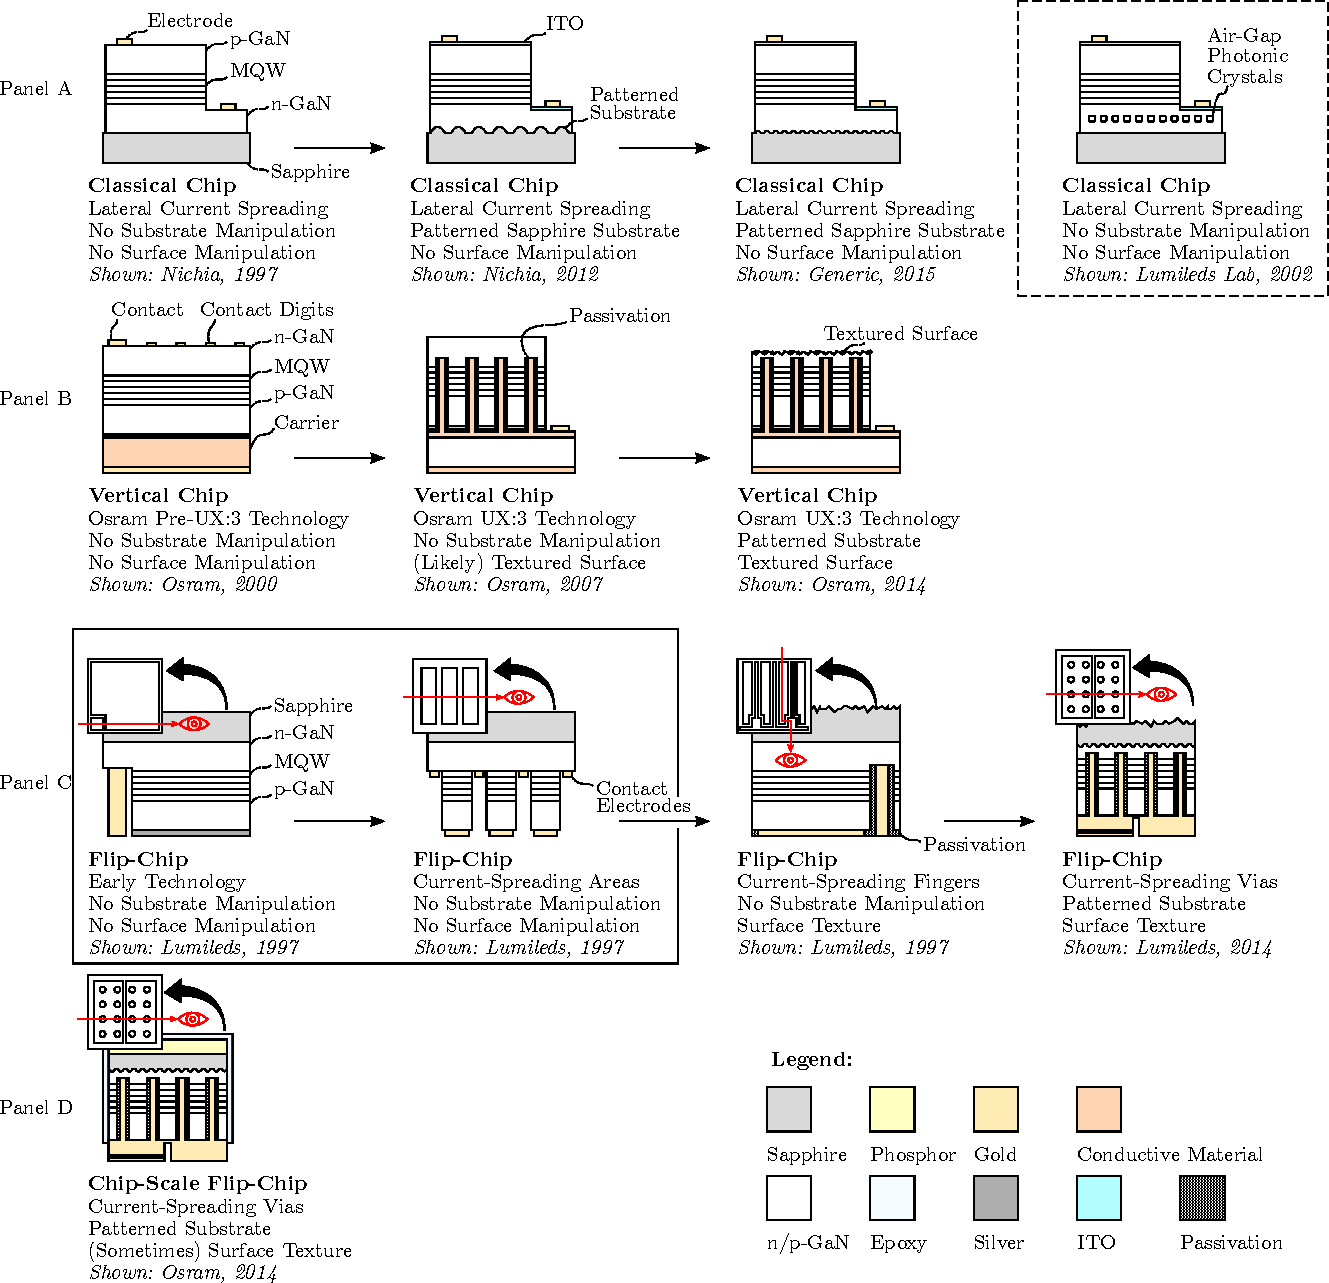
\includegraphics[height=17cm]{2_SSL_EES/article/figures/chip_architecture_overview.pdf}
 \caption{Historical evolution of light-emitting diode chip architectures. Rows from top to bottom: classical chip with lateral current spreading; Osram’s thin GaN flip-chip (vertical) architecture; flip-chip architecture; chip-scale package flip-chip architecture. Shown are side views of chips without packages, along a cutaway line best suited to the features of each architecture. The cutaway surface is indicated by a red arrow with an eye on the overlaid top view of each chip. Note that the dimensions are not to scale, and smaller features are greatly exaggerated for clarity. Years indicated correspond to the earliest identified patent priority date. Black frames around certain designs indicate chip designs not brought to large-scale production. Abbreviations: GaN – Gallium Nitride, ITO – Indium Tin Oxide, MQW – Multiple Quantum Well. Source: adapted and compiled from multiple patents and industry publications. See Supplementary Information, section…, for the full list of sources and references.}
 \label{fgr:chip_architecture_overview}
\end{figure*}


\section{Conclusions}
Our study has analysed in a systematic and granular way the sources of dramatic cost reductions and efficiency improvements in white light-emitting diodes since their introduction to the market in 1996. We find that the total LED device efficiency increased from $5.8\%$ to $38.7\%$ between 2003 and 2020 has been predominantly driven by LED technology innovations that have affected all physical energy loss channels and corresponding device sub-efficiencies. We also find that among those innovations, at least nine were driven by technology originating in areas of science and technology outside LEDs and solid-state lighting—i.e., those nine innovations can be referred to as technology spillovers . These spillovers were responsible for $8.5\%$ of the total efficiency improvements and nearly $100\%$ of the improvements in consumer experience metrics. 

Our manufacturing cost model shows that a $95.5\%$ decrease in the cost of producing white classic-chip LEDs (from $1.11\$$ to $0.05\$$ in 2020 USD) between 2003 and 2020. While efficiency improvements have played an important role in these cost reductions, the largest components of such cost reductions have been driven by increases in the wafer size and yields across different manufacturing steps. In contrast with efficiency improvements, these increases were mainly a result of learning-by-doing and manufacturing equipment improvements rather than LED technology innovations or spillovers. 

Our analysis of the sources, mechanisms and enablers of the identified technology spillovers which were significant drivers of efficiency improvements, highlights the critical role played by a growing deep understanding of the physical, chemical and optical phenomena underlying the operation of LEDs, as well as materials science and technology and nanotechnology involved in the production of LEDs. Specifically, deep physical understanding of LED device efficiency loss channels enabled important breakthroughs and spillovers in LEDs and will enable further innovations to improve LED and SSL efficiency in the future, as expected by eminent experts in the field \cite{Weisbuch2020}. This suggests that additional research in these areas and a more deliberate search for spillovers may accelerate these expected future advances. Our findings on spillover enablers show that these efforts can be further supported or even accelerated by knowledge exchange events and long-term partnerships between academia and industry, dedicated mission-driven public R\&D funding, and freedom of search in academia. This reinforces arguments made against the dichotomy of basic research versus applied research \cite{narayanamurti2016cycles} \cite{narayanamurti2021genesis} and the calls for open, inclusive and flexible research cultures \cite{Stephan2021}.

There are various important avenues of future research that are opened up by our analysis. First, future work could expand the cost model by collecting and including data for a broader set of chip architectures and analyzing the impact of individual innovations and spillovers on costs as opposed to performance. Second, a deeper dive on the role of learning-by-doing is needed both in the cost and performance analysis to identify different types of learning by doing and how it came about. Third, building on the work on LED sub-efficiencies and physical limits, future efforts could focus on identifying priority areas for further efficiency improvements in LEDs and SSL in general. Finally, by comparing the drivers of innovation, technology spillovers, cost reductions and performance improvements at a granular level across different clean energy technologies, we can identify patterns or differences that would help us formulate recommendations for industry and policymakers aimed at accelerating further clean energy innovation for climate change mitigation. 

\section*{Conflicts of interest}
There are no conflicts to declare.

\section*{Acknowledgements}
This research is supported by a grant of the Alfred P. Sloan Foundation titled \href{http://web.archive.org/web/20200623065733/https://sloan.org/grant-detail/8567}{\textit{“What factors drive innovation in energy technologies? The role of technology spillovers and government investment”}}. Michael Weinold further gratefully acknowledges support by the \href{https://www.studienstiftung.ch/}{Swiss Study Foundation}. We would like to thank Venkatesh Narayanamurti, Gabriel Chan, Anna Goldstein, Didier Sornette, and participants of the SPIE West 2021 Conference and \href{https://www.ceenrg.landecon.cam.ac.uk/}{C-EENRG} Seminar Series of the University of Cambridge for many helpful discussions and feedback. We also express our deep gratitude to all interviewees for their willingness to participate in this study and their valuable contributions. Support by German consumer organization \textit{Stiftung Warentest} in providing access to their archive is gratefully acknowledged.

%%%END OF MAIN TEXT%%%

%The \balance command can be used to balance the columns on the final page if desired. It should be placed anywhere within the first column of the last page.

\balance

%If notes are included in your references you can change the title from 'References' to 'Notes and references' using the following command:
%\renewcommand\refname{Notes and references}

%%%REFERENCES%%%
\bibliography{bibliography}
\bibliographystyle{auxiliary/rsc_style_files/bibliography_rsc} %the RSC's .bst file

\end{document}
